\documentclass{article}

\usepackage[utf8]{inputenc}
\usepackage{enumitem}
\usepackage{latexsym}
\usepackage{amsfonts}
\usepackage{amsmath,amssymb,amsthm}
\usepackage{amsfonts}
\usepackage{parskip}
\usepackage{listings}

\usepackage{tikz}
\usetikzlibrary{arrows, automata, bending, positioning}

\newcommand{\set}[1]{\{#1\}}
\newcommand{\Z}{\mathbb{Z}}
\renewcommand{\epsilon}{\varepsilon}

\newenvironment{question}[2]
{
    {\large \textbf{Question #1.}}\\
    #2\\\\
}{\newpage}

\title{Homework 3}
\author{Asier Garcia Ruiz}

\begin{document}
\maketitle

\begin{question}
    {1a}
    {When a PDA transitions, it may push any string over $\Gamma$ onto the stack. Define a 1-PDA to
        be a PDA that, on eack transition, pushed at most one character onto the stack. Show that any PDA
        can be converted to a 1-PDA that recognises the same language.}

    Consider string $s = w_0w_1...w_n$ that is being pushed onto the PDA stack. We create $n-1$
    intermediate states. This results in $n$ total states for the string being pushed. Now, in the
    $i$th state we push the $i$th character of the string and transition to the next state. The
    $n$th state has the same transition function as the state from the orignal PDA that pushes the
    string onto the stack. Therefore, we can turn any PDA into a 1-PDA.
\end{question}

\begin{question}
    {1b}
    {Let us define a context-free grammar $G$ to in "2-form" if, for every nonterminal $A$, there are
        at most two options for replacing $A$ in a derivation.. That is, ther are at most two rules in $G$
        that have $A$ on the left hand side, where the "rule" $A \to B|C|D$ is considered to be three rules.
        Show that, for any context-free grammar, there is a 2-Form context-free grammare that recognises
        the same language.}

    Consider a rule $A \to B_1 | B_2 | \dots | B_n$.
    We change this rule to $A \to B_1 | C_1$ and create $n - 2$ intermediate rules
    \begin{align*}
        C_1     & \to B_2 | C_2     \\
        C_2     & \to B_3 | C_3     \\
                & \vdots            \\
        C_{n-2} & \to B_{n-1} | B_n
    \end{align*}
    If we repeat this process for any rule that has more than two rules, we will end up with a grammar that
    is in 2-form.
\end{question}

\begin{question}
    {1c}{Let $G$ be a context-free grammar for a language $L$, and suppose $L$ contains only strings
        of length  or greater. Prove that there is a context-free grammar $G'$ which generates $L$ such that
        every rule of $G'$ has the form $A \to x_1x_2$ where $A$ is a nonterminal, and each $x_i$ is a
        terminal or nonterminal.}

    Let $G'$ be the Chomsky Normal Form of $G$. We know that every context free language is generated by
    a Chomsky normal form, so this is not as issue to get. This implies we have only three types of rules:
    $A \to BC, A \to a$, and $S \to \epsilon$.

    Now, consider a rule in $G'$ in the form $A \to a$. Then, for every instance of $A$ in the RHS of another rule, we simply
    replace $A$ with $a$. Now, if $A$ has $n$ rules (one of them being the one we just discussed), we create a new rule
    for every of these "extra" rules. Then, for every other rule $S$
    that has $A$ on its RHS we replace $A$ with the corresponding rule. For example,
    if $A \to a$, $A \to XY$, and $S \to AB$, then we would end up with one new rule $D \to XY$ and two rules for $S$, namely $S \to aB$ and $S \to DB$.

    Therefore, every context-free grammar $G$ has a grammar $G'$ that generates the same language and has the given properties.

\end{question}

\begin{question}
    {2a}
    {Give a context-free grammar for the following language
        \[L_1 = \set{a^ib^jc^kd^l | i = j \text{ or } k = l \text{ but not both, } i,j,k,l \geq 0}\]}
    \begin{align*}
        S   & \to S_1 | S_2           \\
        \\
        S_1 & \to AB                  \\
        A   & \to aAb | \epsilon      \\
        B   & \to X_1 | X_2           \\
        X_1 & \to cC | \epsilon       \\
        C   & \to cCd|cC|\epsilon     \\
        X_2 & \to Dd|\epsilon         \\
        D   & \to cDd|Dd|\epsilon     \\
        \\
        S_2 & \to YZ                  \\
        Y   & \to U_1 | U_2           \\
        U_1 & \to aV | \epsilon       \\
        V   & \to aVb|aV|\epsilon     \\
        U_2 & \to Tb | \epsilon       \\
        T   & \to aTb | Tb | \epsilon \\
        Z   & \to cZd|\epsilon
    \end{align*}
\end{question}

\begin{question}
    {2b}
    {Give a context-free grammar for the following language
        \[L_2 = \set{0^i1^j | \text{ for some nonnegative } x,y \in \Z, x + y = i \text{ and } 4x + 3y = j}\]}
    \begin{equation*}
        X \to 0X1111|0X111|\epsilon
    \end{equation*}
\end{question}

\begin{question}
    {3a}
    {Give pushdown automata for the following languages
        $L_4 = \set{w_10w_2 | |w_1| = |w_2|, w_i \in \Sigma^*}$
        the set of string with 0 as the middle character.}

    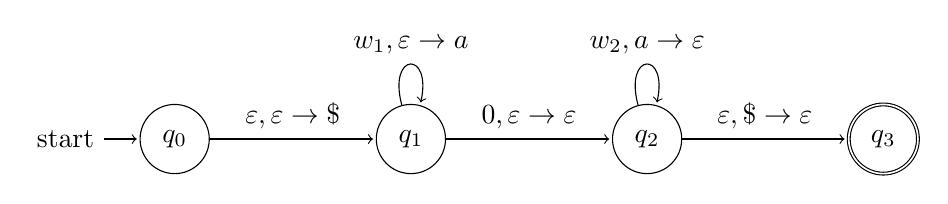
\begin{tikzpicture}[shorten >=1pt,node distance=3cm,on grid,auto]
        \node[state, initial]       (q_0)                                  {$q_0$};
        \node[state]                (q_1)    [right of=q_0]                {$q_1$};
        \node[state]                (q_2)    [right of=q_1]                {$q_2$};
        \node[state, accepting]     (q_3)    [right of=q_2]                {$q_3$};

        \path[->]   (q_0) edge node {$\epsilon, \epsilon \to \$$} (q_1)
        (q_1) edge [loop above] node {$w_1, \epsilon \to a$} ()
        edge node {$0, \epsilon \to \epsilon$} (q_2)
        (q_2) edge [loop above] node {$w_2, a \to \epsilon$} ()
        edge node {$\epsilon, \$ \to \epsilon$} (q_3)
        ;
    \end{tikzpicture}
\end{question}

\begin{question}
    {3a}
    {Give pushdown automata for the following languages
        $L_5 = \set{w | w \text{ is even length, and is not a palindrome}}$
    }
    Let $w = w_1w_2\dots w_i\dots w_n$, $a \in \Sigma, a\neq w_i, b \in \Gamma$.

    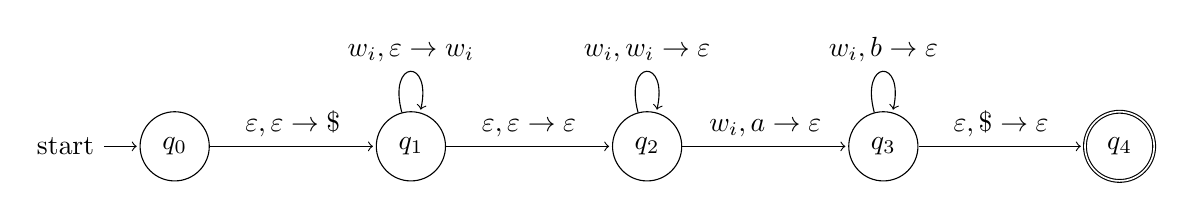
\begin{tikzpicture}[shorten >=1pt,node distance=3cm,on grid,auto]
        \node[state, initial]       (q_0)                                  {$q_0$};
        \node[state]                (q_1)    [right of=q_0]                {$q_1$};
        \node[state]                (q_2)    [right of=q_1]                {$q_2$};
        \node[state]     (q_3)    [right of=q_2]                {$q_3$};
        \node[state, accepting]     (q_4)    [right of=q_3]                {$q_4$};

        \path[->]   (q_0) edge node {$\epsilon, \epsilon \to \$$} (q_1)
        (q_1) edge [loop above] node {$w_i, \epsilon \to w_i$} ()
        edge node {$\epsilon, \epsilon \to \epsilon$} (q_2)
        (q_2) edge [loop above] node {$w_i, w_i \to \epsilon$} ()
        edge node {$w_i, a \to \epsilon$} (q_3)
        (q_3) edge [loop above] node {$w_i, b \to \epsilon$} ()
        edge node {$\epsilon, \$ \to \epsilon$} (q_4)
        ;
    \end{tikzpicture}
\end{question}

\begin{question}
    {4}
    {Show that $L_6 = \set{w | w \text{ is a palindrome which contains an equal number of 0's and 1's}$ is not a context-free using the pumping lemma for
            context free languages.}
        }
        Assume, for the sake of contradiction, that $L_6$ is context-free, and let $p$ be the pumping length. By this assumption, we know that any string $s$ in
    $L_6$ such that $|s| \geq p$ can be split up such that $s = uvxyz$. Furthermore, pumping $uv^ixy^iz$ also gives a string in $L_6$. Now let
    $s = 1^p0^{2p}1^p$. Clearly $|s| \geq p$, so we can split it up into $uvxyz$ such that $|vxy| \leq p$ and $|vy| > 0$. We can also pump it such that
    $uv^ixy^iz \in L_6$ for all $i \geq 0$. This is split up in two cases: $vxy$ contains only 0s and $vxy$ contains at least one 1.

        Suppose that $vxy$ has at least one 1. Then, taking $i = 2$ we see that $uv^2xy^2z \not\in L_6$ since it contains more 1s than 0s. This is a contradiction.

        Suppose that $vxy$ contains only 0s. Then, taking $i = 2$ we see that $uv^2xy^2z \not\in L_6$ since it contains more 0s than 1s. This is a contradiction.

        Therefore, we have shown that $L_6$ is not context free.
\end{question}

\end{document}